\section{Risultati Sperimentali}
\label{sec:Risultati}

In questo capitolo vengono presentati e discussi i risultati ottenuti dall'implementazione dell'algoritmo \emph{Tabu Search} descritto nei capitoli precedenti. Per valutare il comportamento dell’algoritmo, si sono condotti test su diverse istanze del problema, variando i parametri chiave come \emph{tabuTenure}, \emph{maxNoImprovement} e la dimensione dei grafi. I risultati di questi esperimenti sono riportati nella Tabella~\ref{tab:results}, che fornisce un riepilogo compatto delle diverse configurazioni testate e dei rispettivi output ottenuti.

\begin{table}[h]
    \centering
    \small
    \renewcommand{\arraystretch}{1.2}
    \begin{tabular}{cccc||cccc||cccc}
        \toprule
        \textbf{n} & \textbf{m} & \textbf{i} & \textbf{result} & \textbf{n} & \textbf{m} & \textbf{i} & \textbf{result} & \textbf{n} & \textbf{m} & \textbf{i} & \textbf{result} \\
        \midrule
        20 & 60  & 01 & 774  & 20 & 60  & 02 & 1035 & 20 & 60  & 03 & 730  \\
        20 & 60  & 04 & 775  & 20 & 60  & 05 & 871  & 20 & 60  & 06 & 907  \\
        20 & 60  & 07 & 972  & 20 & 60  & 08 & 1085 & 20 & 60  & 09 & 980  \\
        20 & 60  & 10 & 960  & 20 & 120 & 01 & 910  & 20 & 120 & 02 & 1086 \\
        20 & 120 & 03 & 1061 & 20 & 120 & 04 & 1050 & 20 & 120 & 05 & 997  \\
        20 & 120 & 06 & 961  & 20 & 120 & 07 & 1063 & 20 & 120 & 08 & 1162 \\
        20 & 120 & 09 & 1271 & 20 & 120 & 10 & 1133 & 25 & 150 & 01 & 1463 \\
        25 & 150 & 02 & 1132 & 25 & 150 & 03 & 1305 & 25 & 150 & 04 & 1483 \\
        25 & 150 & 05 & 1311 & 25 & 150 & 06 & 1249 & 25 & 150 & 07 & 1589 \\
        25 & 150 & 08 & 1445 & 25 & 150 & 09 & 1366 & 25 & 150 & 10 & 1167 \\
        \hline\hline
        100 & 500  & 01 & 4795 & 100 & 500  & 02 & 5083 & 100 & 500  & 03 & 4705 \\
        100 & 500  & 04 & 4803 & 100 & 500  & 05 & 5225 & 100 & 500  & 06 & 5065 \\
        100 & 500  & 07 & 5050 & 100 & 500  & 08 & 4889 & 100 & 500  & 09 & 4595 \\
        100 & 500  & 10 & 4777 & 100 & 2000 & 01 & 6260 & 100 & 2000 & 02 & 6060 \\
        100 & 2000 & 03 & 5930 & 100 & 2000 & 04 & 6077 & 100 & 2000 & 05 & 6533 \\
        100 & 2000 & 06 & 6158 & 100 & 2000 & 07 & 6568 & 100 & 2000 & 08 & 6379 \\
        100 & 2000 & 09 & 6045 & 100 & 2000 & 10 & 6410 & 200 & 750  & 01 & 9164 \\
        200 & 750  & 02 & 9014 & 200 & 750  & 03 & 9058 & 200 & 750  & 04 & 8330 \\
        200 & 750  & 05 & 9559 & 200 & 750  & 06 & 8626 & 200 & 750  & 07 & 8271 \\
        200 & 750  & 08 & 8835 & 200 & 750  & 09 & 9122 & 200 & 750  & 10 & 8907 \\
        \hline\hline
        200 & 3000 & 01 & 12121 & 200 & 3000 & 02 & 11494 & 200 & 3000 & 03 & 12287 \\
        200 & 3000 & 04 & 13071 & 200 & 3000 & 05 & 11763 & 200 & 3000 & 06 & 11725 \\
        200 & 3000 & 07 & 11985 & 200 & 3000 & 08 & 12042 & 200 & 3000 & 09 & 12203 \\
        200 & 3000 & 10 & 11684 & 800 & 1000 & /  & 46393 &     &      &    &      \\
        \bottomrule
    \end{tabular}
    \caption{Risultati dell'applicazione dell'algoritmo per ogni grafo preso in esame}
    \label{tab:results}
\end{table}

\subsection{Setup Sperimentale}

Le prove sono state eseguite su una macchina con le seguenti specifiche:
\begin{itemize}
    \item \textbf{CPU:} Intel Core i7-1065G7 (1.30\,GHz)
    \item \textbf{RAM:} 16\,GB
    \item \textbf{Sistema Operativo:} WSL Ubuntu 20.04 (64 bit)
    \item \textbf{Linguaggio:} Java (OpenJDK 17)
\end{itemize}

Le istanze di test comprendono grafi con numero di nodi (\(n\)) variabile tra 20 e 800, e numero di archi (\(m\)) tra 60 e 10000. I pesi dei nodi sono interi positivi.

\subsection{Confronto tra Diverse Configurazioni di Parametri}

Per capire come i parametri influenzino le prestazioni, sono state confrontate diverse configurazioni di \emph{tabuTenure} (5, 7), \emph{maxNoImprovement} (10, 20, 30) e \emph{maxIterations} (500, 1000, 2000). In ciascun caso, l'algoritmo è stato eseguito 5 volte su ogni istanza, per ridurre la variabilità stocastica. A titolo di esempio, la tabella~\ref{tab:times} riporta i risultati medi su un insieme di 3 istanze (piccola, media e grande).

\begin{table}[h!]
\centering
\small
\begin{tabular}{l|c|c|c|c|c|c|c}
\hline
\textbf{Config.} & \textbf{n} & \textbf{m} & \textbf{maxIter.} & \textbf{tabuTenure} & \textbf{maxNoImpr.} & \textbf{Time (s)} & \textbf{Results} \\
\hline
C1  & \multirow{6}{*}{20}  & \multirow{6}{*}{60}   & 500  & 5  & 10 & 0.0092  & 774 \\
C4  &  &  & 500  & 7  & 20 & 0.0148  & 774 \\
C7  &  &  & 1000 & 5  & 20 & 0.0156  & 774 \\
C10 &  &  & 1000 & 10 & 30 & 0.021   & 774 \\
C13 &  &  & 2000 & 7  & 10 & 0.0134  & 774 \\
C16 &  &  & 2000 & 10 & 20 & 0.0168  & 774 \\
\hline \hline
C2  & \multirow{6}{*}{100} & \multirow{6}{*}{500}  & 500  & 5  & 10 & 0.0608  & 4795 \\
C5  &  &  & 500  & 7  & 20 & 0.108   & 4795 \\
C8  &  &  & 1000 & 5  & 20 & 0.0836  & 4795 \\
C11 &  &  & 1000 & 10 & 30 & 0.0818  & 4795 \\
C14 &  &  & 2000 & 7  & 10 & 0.062   & 4795 \\
C17 &  &  & 2000 & 10 & 20 & 0.0926  & 4795 \\
\hline \hline
C3  & \multirow{6}{*}{800} & \multirow{6}{*}{10000} & 500  & 5  & 10 & 6.1008  & 46393 \\
C6  &  &  & 500  & 7  & 20 & 6.7292  & 46393 \\
C9  &  &  & 1000 & 5  & 20 & 6.7994  & 46393 \\
C12 &  &  & 1000 & 10 & 30 & 7.2512  & 46393 \\
C15 &  &  & 2000 & 7  & 10 & 6.856   & 46393 \\
C18 &  &  & 2000 & 10 & 20 & 7.54    & 46393 \\
\hline
\end{tabular}
\caption{Risultati medi (5 run) per diverse configurazioni di \emph{maxIterations}, \emph{tabuTenure} e \emph{maxNoImprovement}.}
\label{tab:times}
\end{table}


\noindent
Dall’osservazione dei dati in tabella~\ref{tab:times} emergono due punti essenziali:
\begin{itemize}
    \item \textbf{Dimensioni del grafo come fattore dominante:}
    passando da \((20,60)\) a \((800,10000)\) nodi/archi, si registra un salto netto dei tempi di esecuzione (dall’ordine di microsecondi-millisecondi a svariati secondi).

    \item \textbf{\emph{maxNoImprovement} come parametro più incisivo:}
    a parità di \emph{maxIterations} e \emph{tabuTenure}, valori minori di \emph{maxNoImprovement} (in particolare 10) mostrano i migliori tempi d’esecuzione, mentre configurazioni con \emph{maxNoImprovement} più alto fanno salire i tempi, seppur meno drasticamente del puro aumento di dimensione del grafo.
\end{itemize}

\subsection{Commenti sui Risultati}

Nel complesso, la Tabu Search così configurata è risultata:
\begin{itemize}
    \item \textbf{Affidabile}: produce soluzioni di buona qualità con bassa varianza fra diversi run.
    \item \textbf{Poco sensibile} ai parametri: variazioni dei parametri non cambiano in modo significativo i risultati, come visto in tabella~\ref{tab:times}.
    \item \textbf{Scalabile} fino a grafi di alcune migliaia di archi, con tempi di esecuzione che rimangono in un range accettabile (alcuni secondi).
\end{itemize}

\begin{figure}[h!]
\centering
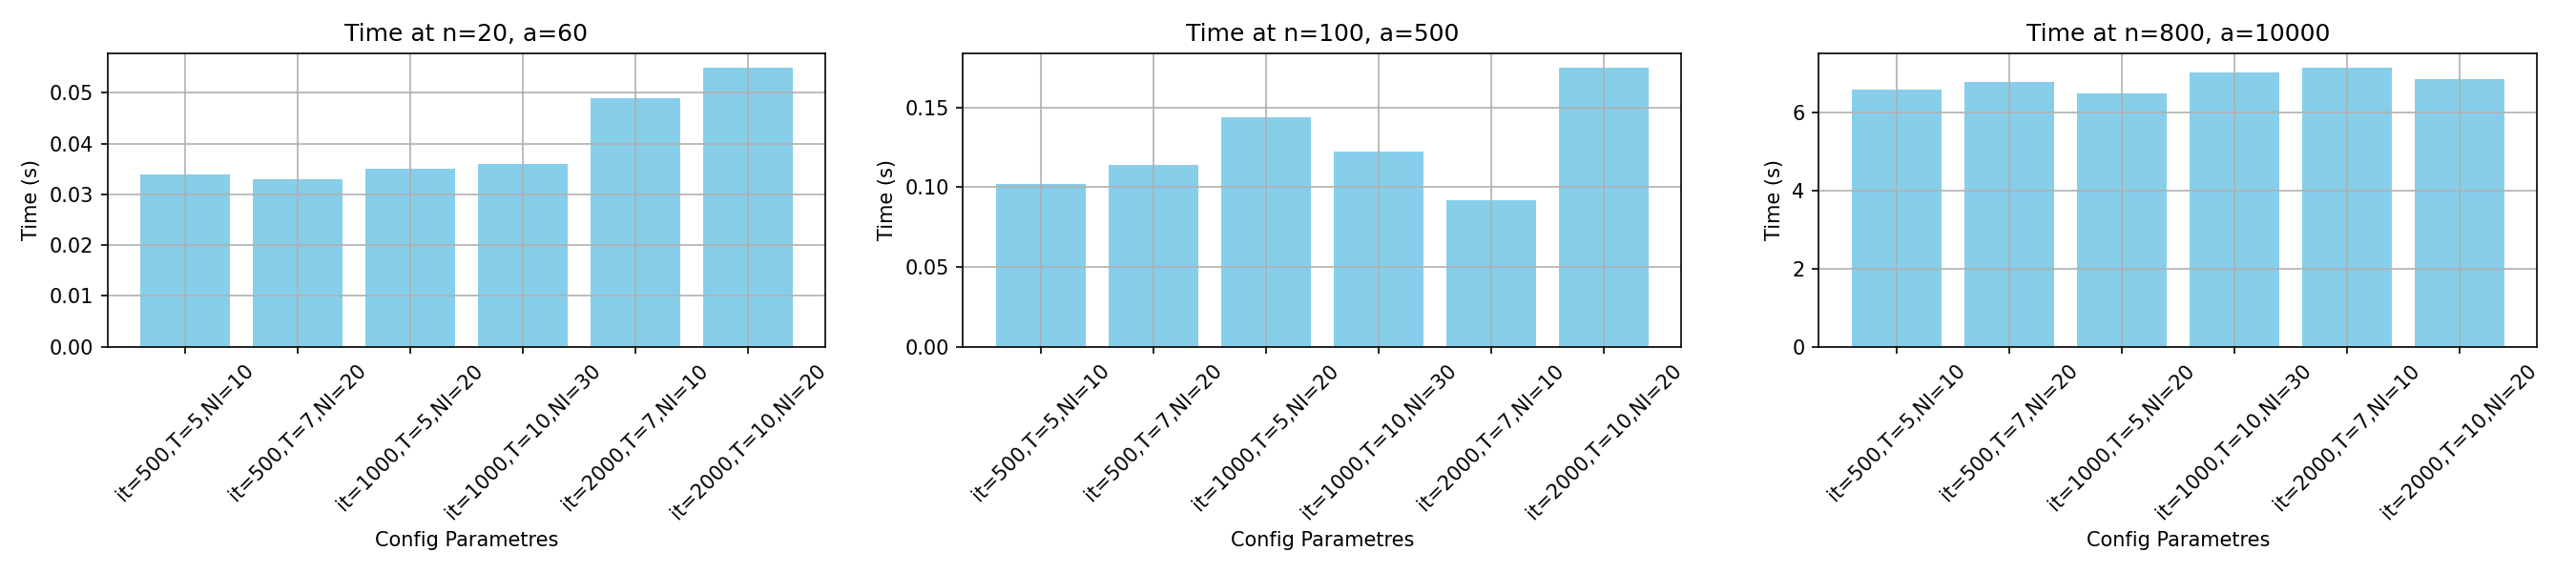
\includegraphics[width=1\textwidth]{images/scalability_plot.png} % Esempio di plot
\caption{Tempo di esecuzione medio in funzione della dimensione del grafo e della configurazione dei tre parametri.}
\label{fig:scalability}
\end{figure}

Una eventuale \emph{long-term memory}, basata sul conteggio di frequenza con cui i nodi appaiono o spariscono dal cover, potrebbe migliorare ulteriormente la diversificazione su istanze molto grandi, sebbene ciò comporti una maggiore complessità implementativa. Nel prossimo capitolo (\ref{sec:Conclusioni}) verranno esposti alcuni spunti di sviluppo e riflessioni conclusive sull'algoritmo e le sue prospettive future.

% Fine capitolo Risultati
